% !TEX TS-program = xelatex
% !TEX encoding = UTF-8 Unicode
\documentclass[10pt,aspectratio=1610]{beamer}
%\documentclass[10pt]{beamer}

\usetheme[progressbar=frametitle]{metropolis}
\usepackage{appendixnumberbeamer}


\usepackage{booktabs}
\usepackage[scale=2]{ccicons}

\usepackage{pgfplots}
\usepgfplotslibrary{dateplot}

\usepackage{xspace}

\usepackage{bm}

% Color definitions 
%\usepackage[dvipsnames]{xcolor}

% Remove "Figure #" from figures
\setbeamertemplate{caption}{\raggedright\insertcaption\par}

% Custom commands
% Metropolis theme name 
\newcommand{\themename}{\textbf{\textsc{metropolis}}\xspace}

% Derivatives
\newcommand{\pfrac}[3][]{\frac{\partial^{#1} #2}{\partial #3^{#1}}}
\newcommand{\dd}[3][]{\frac{\mathrm{d}^{#1} #2}{\mathrm{d} #3^{#1}}}
\newcommand{\pp}[2][]{\partial^{#1}_{#2}}


\newcounter{example}
\stepcounter{example}
\newcounter{exercise}
\stepcounter{exercise}

\renewcommand{\vec}{\mathbf}
\newcommand{\varone}{\vec{x}}
\newcommand{\argone}{(t,\varone)}
\newcommand{\R}{\mathbb{R}}
\newcommand{\CC}{\mathbb{C}}
\newcommand{\Q}{\mathbb{Q}}
\newcommand{\Z}{\mathbb{Z}}
\newcommand{\N}{\mathbb{N}}
\newcommand{\norm}[1]{\left\lVert#1\right\rVert}
\newcommand{\fone}{\vec{f}}
\newcommand{\ftwo}{\vec{g}}
\newcommand{\fthr}{\vec{h}}
\newcommand{\ffor}{\bm{\phi}}
\newcommand{\opone}{\mathcal{L}}
\newcommand{\optwo}{\mathcal{G}}
\renewcommand{\Re}{\operatorname{Re}}
\newcommand{\iprod}[2]{\langle #1,#2 \rangle}
\newcommand{\diff}{\mathrm{d}}
\newcommand{\fouriert}{\mathcal{F}}

\title{Inhomogeneous PDEs revisited}
\subtitle{The inhomogeneous heat and wave equations}
\date{16/3/2021}
\date{}
%\author{18.303 Linear Partial Differential Equations: Analysis and Numerics}
\institute{18.303 Linear Partial Differential Equations: Analysis and Numerics}
\titlegraphic{\hfill
\includegraphics[height=2em]{../MIT-logo.pdf}}

\begin{document}
	
	\maketitle
	
%	\begin{frame}{Table of contents}
%		\setbeamertemplate{section in toc}[sections numbered]
%		\tableofcontents%[hideallsubsections]
%	\end{frame}


\begin{frame}{Basic Notions}
	\begin{columns}[T,onlytextwidth]
		\column{0.46\textwidth}
		Boundary value problems look basically like this:
		\[ 
		\begin{split}
			\opone u(\varone) &= f(\varone), \; \varone \in \omega; \\ 
			\optwo u(\varone) &= g(\varone), \; \varone \in \partial \omega.
		\end{split}
		\]
		
		\onslide*<1>{Now, if $ \fone = 0$, we say that the boundary value problem (the differential equation) is \alert{homogeneous}. Otherwise the problem is said to be \alert{inhomogeneous}.}
		
		\onslide<2->{If the differential operator $ \optwo $ is just a (non-zero) function, these are \alert{Dirichlet boundaries} and $ u $ is equal to some function on the boundary $ \partial \omega $.}
		
		\onslide<3->{If the differential operator is $ \nvec \cdot \nabla = \pfrac{}{\nvec} $ the boundary condition is called \alert{Neumann type} or \alert{flux boundary} condition. This denotes the derivative of function $ u $ in the normal direction of the boundary given by the normal vector $ \nvec (\varone) $ (note that generally it depends on the point $ x \in \partial \omega$).}
		
		\column{0.08\linewidth}
		\column{0.46\textwidth}
		\vspace{4em}
		\begin{figure}
			\centering
			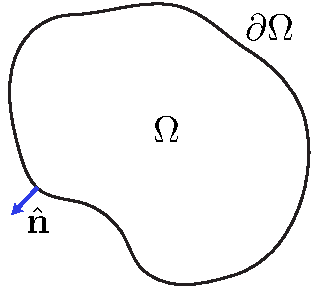
\includegraphics[width=0.8\linewidth]{domain.pdf}
			\caption{An example of a 2d domain and its boundary.}
		\end{figure}
	\end{columns}
\end{frame}

\begin{frame}
	Boundary conditions can be more complicated than Dirichlet or Neumann conditions (and will be e.g. for higher order differential operators). However, we have the following general property:
	
	\pause
	Let $ u_0(\varone) $ solve the \emph{homogeneous} problem
	\[ \begin{split}
		\opone u_0(\varone) &= 0, \; \varone \in \omega; \\ 
		\optwo u_0(\varone) &= g(\varone), \; \varone \in \partial \omega.
	\end{split} \]
	
	\pause
	Now, consider the function $ u(\varone) = v(\varone) + u_0(\varone). $ We have 
	\[ \opone u(\varone) = \opone v(\varone) + \underbrace{\opone u_0 (\varone)}_{=0} = f(\varone). \]
	
	\pause
	We notice that it suffices to require that 
	\[ \optwo v(\varone) = 0,\; \varone \in \partial \omega \]
	because this will make sure that $ \optwo u(\varone) = g(\varone) $, when $ \varone \in \partial \omega $.
\end{frame}

\begin{frame}
	Now we have a boundary value problem 
	\[ \begin{split}
		\opone v(\varone) &= f(\varone), \; \varone \in \omega; \\ 
		\optwo v(\varone) &= 0, \; \varone \in \partial \omega.
	\end{split} \]
	
	This shows us that the general solution can be sought as \\ \alert{the solution to the homogeneous problem with inhomogeneous boundaries} + \alert{the solution to the inhomogeneous problem with homogeneous boundaries}.
\end{frame}


\begin{frame}{Heat equation}
	We have 
	\[  
	\pfrac{}{t} u\argone = \Delta u\argone + f\argone
	\]
	with some spatial boundary conditions for all $ t $ and in addition we are given
	\[  
	u(0,\varone) = u^{(0)}(\varone).
	\]
	
	\pause
	We express $ u $ in the eigenbasis $ \{ \eigtwo \} $ of the Laplacian $ \Delta $ giving
	\[ u\argone = \sum_{\vn} \coefone(t) \eigtwo(\vx).  \]
	
	Similarly,
	\[ f\argone = \sum_{\vn} \coeftwo(t) \eigtwo(\vx).  \] 
\end{frame}

\begin{frame}
	Because the basis is linearly independent, we get 
	\[\pfrac{}{t} \coefone (t) = -\eigvone^2 \coefone(t) + \coeftwo (t). \]
	
	\pause
	Multiplying both sides by $ \exp(\eigvone^2 t ) $ and reorganizing gives
	\[\pfrac{}{t} \coefone (t) e^{\eigvone^2 t} + \eigvone^2 \coefone(t)e^{\eigvone^2 t} =  \coeftwo (t)e^{\eigvone^2 t}. \]
	
	\pause
	We notice that we can write this as 
	\[ \pfrac{}{t} \left( \coefone(t) e^{\eigvone^2 t} \right) = \coeftwo(t) e^{\eigvone^2 t}, \]
	which we can integrate from 0 to t giving 
	\[  \coefone(t) e^{\eigvone^2 t} - \coefone(0) = \int_{0}^{t}\coeftwo(t') e^{\eigvone^2 t'} \diff t'  \]
\end{frame}

\begin{frame}
	We notice that $ \coefone (0) $ is given by the coefficients of the initial condition 
	\[ \coefone (0) = \hat{u}^{(0)}_{\vn}. \]
	
	\pause
	Now we can write the complete solution for the coefficients as 
	\[ \coefone (t) = \hat{u}^{(0)}_{\vn} e^{-\eigvone^2 t} + \int_{0}^{t}\coeftwo(t') e^{-\eigvone^2 (t-t')} \diff t'.  \]
	We see immediately that for $ f=0 $ we get the usual solution to the homogeneous problem.
	
	\pause
	What if $ f $ is independent of time?
\end{frame}

\begin{frame}
	This gives
	\[ 
	\begin{split}
	\coefone (t) &= \hat{u}^{(0)}_{\vn} e^{-\eigvone^2 t} + \coeftwo \int_{0}^{t} e^{-\eigvone^2 (t-t')} \diff t' \\
	& =   \hat{u}^{(0)}_{\vn} e^{-\eigvone^2 t} + \frac{\coeftwo}{\eigvone^2} 
	\left( e^{-\eigvone^2 (t-t')} \right)_{t'=0}^{t} \\
	& = \hat{u}^{(0)}_{\vn} e^{-\eigvone^2 t} + \frac{\coeftwo}{\eigvone^2} 
	\left( 1 - e^{-\eigvone^2 t} \right).
	\end{split}
	\]
	
	\pause
	What if $ t \to \infty $?
	
	\pause
	We obtain the solution to the Poisson equation
	\[ \coefone (t) = \frac{\coeftwo}{\eigvone^2}. \]
\end{frame}

\begin{frame}
	This result is not too surprising if we go back to the original heat equation
	\[ \pfrac{}{t} u\argone = \Delta u\argone + f\argone. \]
	
	\pause
	Just assuming that we will reach a \alert{steady state} with $ \partial_t u = 0 $ gives 
	\[  
	-\Delta u\argone = f\argone.
	\]
\end{frame}

\begin{frame}{Wave equation}
	Now 
	\[ \pfrac[2]{}{t} u\argone = \Delta u\argone + f\argone \]
	with some appropriate boundary conditions and initial conditions
	\begin{align*}
		u(0,\vx) &= \uindex{u}{0}(\vx), \\
		\left( \pfrac{}{t} u\argone \right)_{t=0} &=  \uindex{v}{0}(\vx).
	\end{align*}

	\pause
	We proceed in a same way by writing the equation for the coefficients $ \coefone(t) $ as
	\[ \pfrac[2]{}{t} \coefone(t) = -\eigvone^2 \coefone(t) + \coeftwo (t). \]
	
	\pause
	This is an ordinary differential equation (ODE) but it can be a bit harder to solve.
\end{frame}

\begin{frame}
	Recall that the complete solution is the solution to the homogeneous problem with the necessary initial (boundary) conditions + the solution to the inhomogeneous equation with zero boundaries. 
	
	\pause
	We have already covered the solution to the homogeneous problem (here we write $ h\argone $) and the coefficients are given by
	\[ \coefthr(t) = \alpha_{\vn} \cos(\eigvone t ) + \beta_{\vn} \sin(\eigvone t), \]
	where the coefficients $ \alpha_{\vn} $ and $ \beta_{\vn} $ can be solved from the initial conditions. (For complex equations we have $ \exp(\pm i\eigvone t) $ instead of $ \sin $ and $ \cos $).
	
	\pause
	We can seek the particular solution to the inhomogeneous problem for the coefficients in the form 
	\[ \coeffor(t) = \coeffv (t) \coefthr (t). \]
\end{frame}

\begin{frame}
	Substituting this into the inhomogeneous equation for the coefficients gives 
	\[  
	\begin{split}
		\coeftwo(t) &= 
		\pfrac[2]{}{t} \left(
		\coeffv (t) \coefthr (t)
		\right) + \eigvone^2 \coeffv (t) \coefthr (t) \\
		&= \coeffv''(t) \coefthr + 2 \coeffv'(t) \coefthr'(t) + \coefthr''(t) \coeffv(t) + \eigvone(t)^2 \coefthr(t) \coeffv(t).
	\end{split}
	\]
	
	\pause
	The last two terms solve the homogeneous problem 
	\[ \coeffv(t) \underbrace{\left( \coefthr''(t)  + \eigvone(t)^2 \coefthr(t) \right)}_{=0}. \]
	
	\pause
	This gives 
	\[ \coeffv''(t) \coefthr(t) + 2 \coeffv'(t) \coefthr'(t) = \coeftwo (t). \]
	
	\pause
	Multiplying by $ \coefthr  $ gives 
	\[ \coeffv''(t) \coefthr(t)^2 + 2 \coeffv'(t) \coefthr'(t)\coefthr(t) = \coeftwo (t)\coefthr(t), \]
	which we can write as
	\[ \pfrac{}{t} \left( \coeffv'(t)  \coefthr(t)^2 \right) = \coeftwo (t)\coefthr(t). \]
	
\end{frame}

\begin{frame}
	Now this can be integrated from 0 to $ t $  giving
	\[ \coeffv'(t)  \coefthr(t)^2 - \coeffv'(0)  \coefthr(0)^2  = \int_{0}^{t} \coeftwo (t')\coefthr(t') \diff t'.  \]
	
	\pause
	\textbf{Question:} we know what $ \coefthr(0) $ from the initial conditions but what is $ \coeffv'(0) $ (or $ \coeffv(0)  $)?
	
	\pause
	They have to be 0 since the complete solution was the solution to the homogeneous problem with the given boundaries + the particular inhomogeneous solution with zero boundaries.
	
	\pause
	Now we can write the formal solution for the coefficients as 
	\[\coeffor(t) =  \coefthr(t) \coeffv(t) = \int_{0}^{t} \int_{0}^{t'}\coeftwo (t'') \frac{\coefthr(t)\coefthr(t'')}{\coefthr(t')^2} \diff t'' \diff t'  \]
	
	\pause
	and the complete solution is 
	\[ \coefone (t) = \coefthr(t) + \coeffor(t).  \]
\end{frame}

\begin{frame}{The other way}
	That all seemed somewhat complicated so let's do something else. For the coefficients of the particular solution we have 
	\[ \pfrac[2]{}{t} \coeffor (t) + \eigvone^2 \coeffor(t) = \coeftwo (t). \]
	
	\pause
	It turns out that the calculation of the Fourier coefficients can be extended to infinity and the function $ \coeffor $ can be expressed as 
	\[ \coeffor(t) = \frac{1}{2\pi} \int_{-\infty}^{\infty} \hat{P}_{\vn} (\omega) e^{i\omega t} \diff \omega. \]
	(Note that now $ \omega $ is a continuous variable.)
	
	\pause
	The function $ \hat{P}_{\vn} $ can be obtained as 
	\[ \hat{P}_{\vn} = \int_{-\infty}^{\infty} \coeffor(t) e^{-i\omega t} \diff t. \]
	
	\pause
	This is the actual \alert{Fourier transform} and here we have also defined the inverse transform. 
\end{frame}

\begin{frame}
	We will write the coefficients using the Fourier expression giving the equation
	\[  \pfrac[2]{}{t} \int_{-\infty}^{\infty} \hat{P}_{\vn} (\omega) e^{i \omega t} \diff \omega  
	+  \int_{-\infty}^{\infty} \eigvone^2 \hat{P}_{\vn} (\omega) e^{i \omega t} \diff \omega 
	=  \int_{-\infty}^{\infty}  \hat{F}_{\vn} (\omega) e^{i \omega t} \diff \omega. 
	\]
	
	\pause
	Taking the derivative inside the integral gives 
	\[ - \int_{-\infty}^{\infty} \omega^2 \hat{P}_{\vn} (\omega) e^{i \omega t} \diff \omega  
	+  \int_{-\infty}^{\infty} \eigvone^2 \hat{P}_{\vn} (\omega) e^{i \omega t} \diff \omega 
	=  \int_{-\infty}^{\infty}  \hat{F}_{\vn} (\omega) e^{i \omega t} \diff \omega. 
	\]
	
	\pause
	It turns out that the functions $ \exp(i \omega t ) $ form an orthogonal basis implying that the coefficients have to be the same. This gives 
	\[ -\omega^2 \hat{P}_{\vn} (\omega) + \eigvone^2 \hat{P}_{\vn} (\omega) e^{i \omega t} 
	= \hat{F}_{\vn} (\omega).
	\]
\end{frame}

\begin{frame}
	Solving for $ \hat{P}_{\vn} $ gives
	\[ \hat{P}_{\vn} (\omega) = \frac{\hat{F}_{\vn} (\omega)}{\eigvone^2 - \omega^2}. \]
	
	\pause
	We can use this to solve for $ \coeffor $ resulting in
	\[ \coeffor (t) = \frac{1}{2\pi} \int_{-\infty}^{\infty} \frac{\hat{F}_{\vn}(\omega)}{\eigvone^2 - \omega^2} e^{i \omega t}  
	\diff \omega.
	\]
	
	\pause
	What if $ \hat{F}_{\vn} (\eigvone) $ is not zero? Does the integral diverge? 
	
	\pause
	That is something that is called a \alert{resonance} but that will be a story for another day...
\end{frame}

\end{document}
